%!TeX root=../tese.tex
%("dica" para o editor de texto: este arquivo é parte de um documento maior)
% para saber mais: https://tex.stackexchange.com/q/78101

%% ------------------------------------------------------------------------- %%

% "\chapter" cria um capítulo com número e o coloca no sumário; "\chapter*"
% cria um capítulo sem número e não o coloca no sumário. A introdução não
% deve ser numerada, mas deve aparecer no sumário. Por conta disso, este
% modelo define o comando "\chapter**".
\chapter**{Introduction}
\label{cap:introduction}

\en

The Linux kernel is a widely used Free/Libre/Open Source Software (FLOSS) project, 
powering 96.3\% of the top one million web servers and 85\% of smartphones worldwide. 
Maintaining the kernel is an enormous task, involving more than 28 million lines of 
code and contributions from over twenty thousand developers
\footnote{Data directly extracted from Linux github repository \citep{linuxrepo}.
Counted  28783390 lines of code and 20699 number of contributors in May 29th, 2025.
Number of contributors counted as number of unique full name listed as author of a patch.}.
Due to the scale of the project, not all contributions adhere to best practices, resulting 
in poor-quality code artifacts that may complicate maintenance and future feature development.

One such artifact is code duplication, which is the focus of this research. The motivation for 
this work began with a practical problem rooted in device drivers, which are a major part 
of the kernel, representing 66\% of the source code\citep{marcelo}. We interacted with the 
maintainers of the AMD Display driver, an essential component for the 19\% of personal GPUs 
manufactured by AMD in 2023\citep{gpumarket}. They shared their challenges with a significant 
amount of duplicated code that hampers the driver's maintenance. In searching for a solution, 
we found that existing tools are not well-suited for identifying duplications in large-scale 
codebases like the Linux kernel, nor do they offer guidance on how to resolve the duplications 
they find. Despite searching both formal and grey literature, existing solutions fell short of 
addressing these specific challenges. The list of related tools examined in this exploratory 
research is available in Appendix \ref{app:gray}.

This research presents ArKanjo, a command-line tool designed to detect and analyze function-level 
duplications in the Linux kernel. Released under the MIT license, ArKanjo uses a two-stage 
architecture with a Preprocessor and a Query Responder. This design separates the heavy 
computational analysis from the fast querying of duplication results, making it effective for 
large codebases. We validated the tool by comparing its results with the BigCloneBench dataset
\citep{bigclonebench} and by conducting an empirical analysis on a randomly selected set of 
files from the AMD Display driver.

Beyond detection, we also investigated if the duplications found by ArKanjo could be mitigated.
This was achieved through an ethnographic approach, which included a participant observation 
study where we attempted to mitigate duplications, and a non-participant observation study of 
university students tasked with fixing duplications found by the tool. These studies showed that 
ArKanjo can effectively lower the barrier for new contributors, as evidenced by its role in 
guiding students to make their first code contributions to the kernel.

\section**{Research Design}

\label{sec:intresearch}

To address the code duplication problem within the Linux kernel, this research employs a 
multi-method approach designed to bridge the gap between detection and practical mitigation. 
Our approach, illustrated in Figure \ref{fig:reDesign}, is structured into two interconnected phases that progress 
from tool development to an in-depth study of its application within the kernel’s development community. 
The overall objective is to produce not only a functional tool but also actionable insights into 
the patterns and practices surrounding code duplication and its resolution.

\begin{figure}[h]
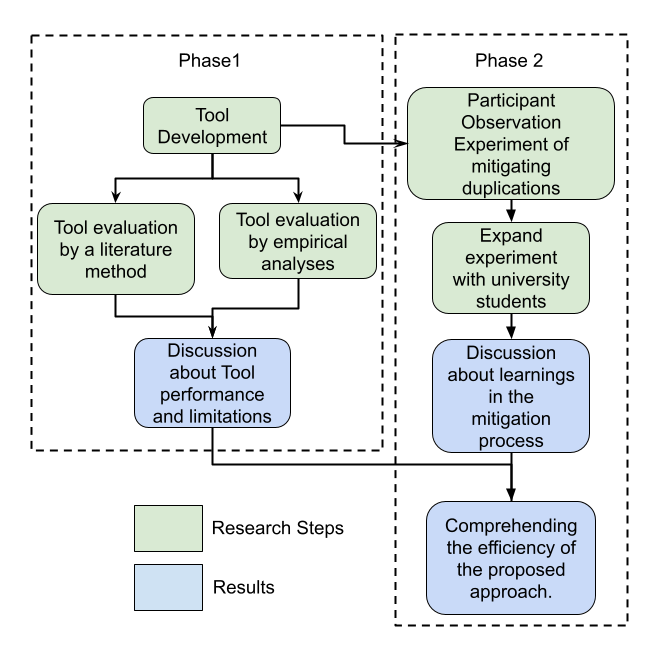
\includegraphics[scale=0.9]{research_design}
\caption{Diagram of the research design.}
\label{fig:reDesign}
\end{figure}

The initial phase of our research focused on the development and validation of ArKanjo, a 
command-line tool capable of identifying code duplication at the function level.  The 
tool's accuracy was rigorously validated by evaluating its performance against the 
standard BigCloneBench dataset \citep{bigclonebench} and by conducting an empirical analysis 
of its results within the AMD Display driver.  This foundational work ensured we had a 
reliable instrument to proceed with the practical investigation of code duplication 
in our target subsystems.

With a validated tool, the research then moved from detection to practice, investigating 
the real-world challenges of mitigating the identified duplications. This was accomplished 
through an ethnographic study designed to engage with the kernel community and understand 
their perspectives on code quality and refactoring.  This study had two components: a 
participant-observation experiment where the author submitted refactoring patches to the 
AMD Display driver, and a non-participant observation of university students using ArKanjo 
to contribute fixes to both the AMD Display and Industrial I/O subsystems.  

By combining tool 
development with direct community interaction, this research design allows for a comprehensive 
understanding of the technical and social factors that influence the mitigation of duplicated 
code in a large-scale open-source project.

\section**{Thesis Structure}

This manuscript consists of five more chapters. Chapter \ref{cha:back} presents
the literature overview for code duplication detection (main definitions,
current approaches in the literature), a brief description of the Linux kernel and the components
explored in this work, 
and a review of refactoring methods used throughout this research. Chapter
\ref{cha:tool} presents ArKanjo, our proposed tool to detect code duplication, 
describing all the main components.  Chapter \ref{cha:method}
describes the research methods selected to guide our work. Chapter
\ref{cha:results} shows the results we had through our work, from the research methods to 
evaluate our tool and the ethnographic studies. Chapter \ref{cha:conclusion} concludes this research.

